%
% Geschlossene 1-Formen und Wegunabhängigkeit
%
\section{Geschlossene 1-Formen und Wegunabhängigkeit
\label{buch:green:section:geschlossen}}
Für die 1-Formen $df$ ist die Berechnung des Wegintegrals besonders
einfach, da $f$ als ``Stammfunktion'' betrachtet werden kann.
Nicht jede 1-Form lässt sich als Differential einer Funktion $df$ 
schreiben.
In diesem Abschnitt soll ein Kriterium dafür gefunden werden, 
ob eine 1-Form $\alpha$ als $\alpha=df$ geschrieben werden kann.

%
% Äusseres Differential von $df$
%
\subsection{Äusseres Differential von $df$}
Ist $f$ eine Funktion auf der Mannigfaltigkeit $M$, dann können wir
die 1-Form $\alpha = df$ bilden.
In einer Karte ist $\alpha$ durch die partiellen Ableitungen
\[
\alpha
=
\sum_{i=1}^n
\frac{\partial f}{\partial x^i}(x)\,dx^i
\]
gegeben.
Für die äussere Ableitung von $df$, bildet man
\[
d\alpha
=
\sum_{i,k=1}^n
\frac{\partial}{\partial x^k}
\frac{\partial f}{\partial x^i}(x)\,
dx^k
\wedge
dx^i.
\]
Die Terme mit $i=k$ sind Vielfache von $dx^i\wedge dx^i=0$, tragen
also nichts bei.
In der Summe (man beachte die einsteinsche Summenkonvention)
tritt jedes Paar von verschiedenen Indizes genau zweimal in verschiedener
Reihenfolge auf, wegen $dx^i\wedge dx^k = - dx^k \wedge dx^i$ kann man
\begin{align}
d\alpha
&=
\sum_{i < k}
\biggl(
\frac{\partial^2 f}{\partial x^i\,\partial x^k}(x)\, dx^i\wedge dx^k
+
\frac{\partial^2 f}{\partial x^k\,\partial x^i}(x)\, dx^k\wedge dx^i
\biggr)
\notag
\\
&=
\sum_{i < k}
\biggl(
\frac{\partial^2 f}{\partial x^i\,\partial x^k}(x)
-
\frac{\partial^2 f}{\partial x^k\,\partial x^i}(x)
\biggr)
\, dx^i\wedge dx^k
\label{buch:green:geschlossen:eqn:dalpha}
\end{align}
schreiben.
Da $f$ beliebig oft stetig differenzierbar sind, sind die partiellen
Ableitungen vertauschbar, der Klammerausdruck in
\eqref{buch:green:geschlossen:eqn:dalpha}
verschwindet und es folgt $d\alpha = 0$.

\begin{definition}[Geschlossene 1-Form]
\index{geschlossene 1-Form}%
Eine 1-Form $\alpha$ heisst {\em geschlossen}, wenn ihr äusseres
Differential $d\alpha=0$ verschwindet.
\end{definition}

Es liegt nahe zu vermuten, dass jede geschlossene 1-Form als Differential
geschrieben werden kann.
Dies ist jedoch nicht richtig, wie das folgende Beispiel zeigt.

\begin{beispiel}
\label{buch:green:geschlossen:beispiel:wegabhaengig}
Wir betrachten die 1-Form
\[
\alpha
=
\frac{-y}{x^2+y^2}\,dx
+
\frac{x}{x^2+y^2}\,dy
\]
auf $M=\mathbb{R}^2\setminus\{0\}$.
Die äussere Ableitung ist
\begin{align*}
d\alpha
&=
\frac{\partial}{\partial y}
\frac{-y}{x^2+y^2}
\,dy\wedge dx
+
\frac{\partial}{\partial x}
\frac{x}{x^2+y^2}
\,dx\wedge dy
\\
&=
\biggl(
\frac{\partial}{\partial y}
\frac{y}{x^2+y^2}
+
\frac{\partial}{\partial x}
\frac{x}{x^2+y^2}
\biggr)
\,dx\wedge dy.
\intertext{Die beiden Ableitungen gehen durch Vertauschen von $x$ und $y$
ineinander über.
Sie können leicht mit Maxima oder einem anderen Computeralgebraprogramm
berechnet werden und sind}
&=
\biggl(
\frac{x^2-y^2}{(x^2+y^2)^2}
+
\frac{y^2-x^2}{(x^2+y^2)^2}
\biggr)
\,dx\wedge dy
=
0,
\end{align*}
$\alpha$ ist also eine geschlossene 1-Form.

Allerdings lässt sich $\alpha$ nicht als Differential schreiben.
Dann liessen sich nämlich die Wegintegrale für die Halbkreise
\begin{align*}
\gamma_+&\colon [0,\pi] \to \mathbb{R}^2 : t \mapsto (\cos t,\sin t)
\\
\gamma_-&\colon [0,\pi] \to \mathbb{R}^2 : t \mapsto (\cos t,-\sin t)
\end{align*}
von $(1,0)$ nach $(-1,0)$ in der oberen bzw.~der unteren Halbebene
einfach als Differenz der Funktionswerte berechnen, sie müssten
also gleich sein.
% XXX Graphik für die Definition der Wege \gamma_+ und \gamma_-
Wir berechnen daher die beiden Wegintegrale:
\begin{align*}
\int_{\gamma_+}\alpha
&=
\int_{0}^{\pi}
\frac{-\sin t}{\cos^2 t+\sin^2t}(-\sin t)
+
\frac{\cos t}{\cos^2 t+\sin^2t}\cos t
\,dt
\\
&=
\int_0^\pi \sin^2 t+\cos^2 t\,dt
=
\int_0^\pi 
\,dt
=
\pi,
\\
\int_{\gamma_-}\alpha
&=
\int_{0}^{\pi}
\frac{-(-\sin t)}{\cos^2 t+\sin^2t}(-\sin t)
+
\frac{\cos t}{\cos^2 t+\sin^2t}(-\cos t)
\,dt
\\
&=
-\int_0^\pi \sin^2 t+\cos^2 t\,dt
=
-\int_0^\pi 
\,dt
=
-\pi.
\end{align*}
Da die beiden Wegintegrale verschieden sind, kann $\alpha$ kein
Differential sein.
\end{beispiel}

%
% Wegunabhängigkeit
%
\subsection{Wegunabhängigkeit}
Das Beispiel \ref{buch:green:geschlossen:beispiel:wegabhaengig}
verrät auch, warum die Vermutung falsch ist.
Wenn $\alpha=df$ ist, dann liefert jeder Weg zwischen zwei Punkten
$A$ und $B$ den gleichen Wert $f(B)-f(A)$ des Wegintegrals von $\alpha$.
Tatsächlich geben im Beispiel Wege auf verschiedenen Seiten des Nullpunktes
verschiedene Werte des Wegintegrals.
Die Vermutung kann also nur stimmen, wenn diese Situation ausgeschlossen
werden kann.

\begin{definition}[Einfach zusammenhängend]
Eine Mannigfaltigkeit heisst {\em einfach zusammenhängend}, wenn sich
\index{einfach zusammenhangend@einfach zusammenhängend}
jeder geschlossene Weg differenzierbar in einen Punkt zusammenziehen
lässt.
\end{definition}

Eine Mannigfaltigkeit ist insbesondere einfach zusammenhängend, wenn
die ganze Mannigfaltigkeit in einen Punkt zusammenziehbar ist.
%
% fig-homotopie.tex
%
% (c) 2025 Prof Dr Andreas Müller
%
\begin{figure}
\centering
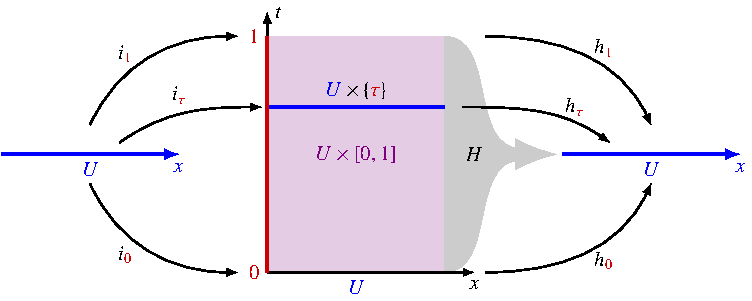
\includegraphics{chapters/060-pformen/images/homotopie.pdf}
\caption{Eine Homotopie $H$ ist eine Abbildung $U\times[0,1]$, die
die Abbildung $h_0\colon U\to U$ in die Abbildung $h_1\colon U\to U$
deformiert.
Die Abbildung $h_{\tau}$ entsteht durch Einsetzen des Wertes $\tau$
in das zweite Argument von $H$, was gleichbedeutend ist mit der
Zusammensetzung von $H$ mit $i_\tau$: $h_\tau=H\circ i_\tau$.
\label{buch:pformen:fig:homotopie}}
\end{figure}
%
Die Abbildung
\[
H
\colon
\mathbb{R}^n\times [0,1]
:
(x,t) \mapsto H_t(x) = (1-t)x
\]
deformiert die identische Abbildung
\(
H_0(x)
=
x
\)
in die Nullabbildung
\(
H_1(x) = 0
\).
Indem man den Parameter $t$ von $0$ auf $1$ anwachsen lässt, werden
alle Punkte in den Nullpunkte gezogen.
Ein geschlossener Weg $\gamma(s)$ wird dabei differenzierbar in
den konstanten geschlossenen Weg $H_1(\gamma(s))=0$ zusammengezogen.
Ein Abbildung dieser Art heisst eine {\em Homotopie}
\index{Homotopie}%
der identischen Abbildung in die Nullabbildung.

\begin{definition}[differenzierbare Homotopie]
Eine differenzierbare Homotopie zweier Wege $\gamma_0$ und $\gamma_1$
in der differenzierbaren Manigfaltigkeit mit den gleichen Endpunkten
ist eine differenzierbare Abbildung
\[
H
\colon
[0,1]\times[0,1]
\to
M
\]
mit
\[
\left.
\begin{aligned}
H_0(s) &= \gamma_0(s)\\
H_1(s) &= \gamma_1(s)
\end{aligned}
\;
\right\}
\qquad\text{und}\qquad
\left\{\;
\begin{aligned}
H_t(0) &= \gamma_0(0) = \gamma_1(0) = A\\
H_t(1) &= \gamma_0(1) = \gamma_1(1) = B.
\end{aligned}
\right.
\]
Wege, die durch eine differenzierbare Homotopie verbunden sind,
heissen {\em homotop} (Abbildung~\ref{buch:green:fig:homotopie}).
\end{definition}

Die Kugeloberfläche $S^2$ ist einfach zusammenhängend, zum Beispiel
kann man den Äquator im Nullpunkt zusammenzieht.
Es gibt aber im Gegensatz zum Beispiel $\mathbb{R}^n$ keine Homotopie
der identischen Abbildung der Kugeloberfläche in eine konstante
Abbildung.

\begin{satz}
\label{buch:green:geschlossen:satz:wegunabhaengig}
Für eine geschlossene 1-Form $\alpha$ ist das Integral
\[
\int_{\gamma_0}\alpha = \int_{\gamma_1} \alpha
\]
über zwei homotope Wege $\gamma_0$ und $\gamma_1$ gleich.
\end{satz}

\begin{proof}
Wir betrachten die Homotopie $H:[0,1]\times[0,1]\to M$ zwischen
den beiden Wegen.
Dann ist nach dem Satz von Green
\[
\int_{[0,1]\times[0,1]}
TH^*(d\alpha)
=
\int_{\partial [0,1]^2} TH^*(\alpha).
\]
Wegen $d\alpha=0$ verschwindet das Integral auf der linken Seite.
Das Integral auf der rechten Seite setzt sich aus vier Wegintegralen
zusammen, einem für jede Kante des Quadrates $\partial[0,1]^2$.
Das Integral entlang der Seite $[0,1]\times\{0\}$ ergibt das Integral
entlang dem $H_0(s) = \gamma_0(s)$.
Die Kante $[0,1]\times\{1\}$ ergibt das Integral entlang der
Kurve $H_1(s) = \gamma_1(s)$, allerdings wird der Weg in umgekehrter
Richtung durchlaufen.
Die beiden Kanten $\{0\}\times[0,1]$ und $\{1\}\times[0,1]$ sind
konstant, das Integral entlang dieser Kanten ist daher $0$.
Von den Wegintegralen bleiben daher
\[
0
=
\int_{\partial[0,1]^2} (TH)^*(\alpha)
=
\int_{\gamma_0} \alpha
-
\int_{\gamma_1} \alpha
\quad\Rightarrow\quad
\int_{\gamma_0} \alpha
=
\int_{\gamma_1} \alpha.
\]
Die beiden Wegintegrale sind gleich.
\end{proof}

Im Beispiel~\ref{buch:green:geschlossen:beispiel:wegabhaengig}
war zwar $d\alpha=0$ aber es gab keine Homotpie, die die Wege
entlang dem Einheitskreis vom Punkt $(1,0)$ zum Punkt $(-1,0)$
in der oberen bzw.~der unteren Halbebene verbindet.

%
% Geschlossene 1-Formen auf einfach zusammenhängenden Gebieten
%
\subsection{Geschlossene 1-Formen auf einfach zusammenhängenden Gebieten}
Die Wegunabhängigkeit des Wegintegrals für eine geschlossene 1-Form
kann jetzt verwendet werden, um eine Funktion $f$ zu finden, deren
Differential die gegebene 1-Form ist.

\begin{satz}
\label{buch:green:geschlossen:satz:poincare}
Eine geschlossene 1-Form $\alpha$ auf einem einfach zusammenhängenden
Gebiet kann als $\alpha=df$ geschrieben werden.
\end{satz}

Die nach Satz~\ref{buch:green:geschlossen:satz:poincare}
existierende Funktion $f$ ist nicht eindeutig, denn mit $f$ hat
auch $f+c$ für jede Konstante $c\in\mathbb{R}$ das Differential
\[
d(f+c) = df + dc = df = \alpha.
\]
Der Beweis wird klar machen, was die Bedeutung

\begin{proof}
Sie $\alpha$ eine geschlossene 1-Form auf der einfach zusammenhängenden
Mannigfaltigkeit $M$.
Ausserdem wird ein Punkt $A\in M$ gewählt.
Für jeden Punkt $P\in M$ wählen wir einen Weg $\gamma:\colon[0,1]\to M$,
der $A$ mit $P$ verbindet.
Die Funktion $f\colon M\to\mathbb{R}$ wird als
\[
f(P) = \int_{\gamma} \alpha.
\]
Nach Satz~\ref{buch:green:geschlossen:satz:wegunabhaengig} ist das eine
konsistente Definition, denn jede Wahl des Weges ergibt den gleichen
Wert des Integrals.
Wir müssen nachprüfen, dass $df=\alpha$ ist.

Um die Ableitung zu berechnen, verwenden wir eine Karte, in der sich die
1-Form als
\[
\alpha = a_i(x)\, dx^i
\]
schreiben lässt.
Wir müssen zeigen, dass
\[
a_i(x) = \frac{\partial f}{\partial x^i}(x)
\]
ist.
Dazu verwenden wir nochmals die Möglichkeit, den Weg $\gamma$ frei wählen
zu können.
Wir wählen in so, dass $\gamma(1)=x$ ist und
\[
\dot{\gamma}(1) = e_i
\]
der Standardbasisvektor ist.
Nach Definition der Funktion $f$ ist
\[
\frac{d}{dt}
f(\gamma(t))
\biggl|_{t=1}
=
\langle
\alpha,
e_i
\rangle
=
a_i(x).
\]
Da dies für jede andere Koordinate auch gilt, folgt $df=\alpha$.
\end{proof}

Im Beweis wurde stillschweigend angenommen, dass sich für jedes
Paar von Punkten in der Mannigfaltigkeit ein Weg finden lässt, der
die beiden Punkte verbindet.
Nicht jede Mannigfaltigkeit hat diese Eigenschaft.
Die Oberflächen der Planeten des Sonnensystems sind zweidimensionale
Mannigfaltigkeiten $S^2$, auf jeder einzelnen sind Punkte untereinander
verbindbar.
Es gibt aber keine Wege zwischen den einzelnen Planeten.
Man nennt eine Mannigfaltigkeit {\em wegzusammenhängend}, wenn es zu jedem
Paar von Punkten einen verbindenden Weg gibt.

Der Beweis ist also nur korrekt für wegzusammenhängende Mannigfaltigkeiten.
Trotzdem gilt der Satz allgemein.
Dazu beginnt man mit einem Punkt $A_0\in M$ und berechnet die Funktion $f$
für jeden Punkt $P\in M$ der sich mit $A_0$ verbinden lässt.
Damit ist $f$ auf der sogenannten {\em Wegzusammenhangskomponente} von $A_0$
definiert.
Die Zusammenhangskomponente ist eine Untermannigfaltigkeit von $M$.
Falls sie nicht ganz $M$ umfasst, wählen wir einen weiteren Punkt $A_1$,
der nicht mit $A_0$ verbunden werden kann, und definieren $f$ auf der
Wegzusammenhangskomponente von $A_1$.
Auf diese Weise lässt sich die Funktion in jeder Wegzusammenhangskomponente
definieren.

Eine andere Wahl des Starpunktes $A_k$ in jeder Wegzusammenhangskomponente
verändert die Werte der Funktion $f$ in der Zusammenhangskomponente
um eine Konstante $c_k$.
Die Funktion $f$ ist daher nur bis auf eine Konstante $c_k\in\mathbb{R}$
in jeder Zusammenhangskomponente definiert.

%
% Potentialfelder
%
\subsection{Potentialfelder}
Das Gravitationsfeld ist bekannt dafür, dass die Arbeit, die gegen
das Feld geleistet werden muss, um einen Massepunkt von einem Punkt $A$
zu einem Punkt $B$ zu bewegen, nicht von der Wahl des Weges abhängt.
Die Unabhängigkeit vom Weg garantiert, dass es
eine Funktion $U(x)$ gibt, mit der man den Energieunterschied
$U(B)-U(A)$ berechnen kann.
Die Funktion $U$ heisst das Potential.
In der Physik wird es meistens noch durch die Masse geteilt,
diese Unterscheidung ist für die aktuelle Diskussion jedoch unwichtig.

Sei $\gamma(t)$ die Kurve, auf der sich der Massepunkt 
bewegt.
Die Leistung gegen das Gravitationsfeld ist dann
$\langle dU, \dot{g}(t)\rangle$.
Die Funktion $U$ kann als Wegintegral von $dU$ rekonstruiert werden.

\begin{definition}[Potential]
Eine 1-Form $\omega$ heisst ein {\em Potentialfeld}, wenn es eine
Funktion $U$ gibt derart, dass $dU=\omega$.
\end{definition}

Nach Satz~\ref{buch:green:geschlossen:satz:poincare} ist $\omega$
auf einem einfach zusammenhängenden Gebiet genau dann ein Potentialfeld,
wenn $d\omega=0$ ist.

\begin{beispiel}
Für das Gravitationsfeld einer Masse $M$ im Nullpunkt des Koordinatensystems
ist die potentielle Energie
\[
U(x,y,z)
=
-\frac{GM}{r}.
\]
Die äussere Ableitung 
\begin{align*}
dU
&=
\frac{\partial U}{\partial x}\,dx
+
\frac{\partial U}{\partial y}\,dy
+
\frac{\partial U}{\partial z}\,dz
\\
&=
-\frac{GM}{r^3}\bigl(
x\,dx
+
y\,dy
+
z\,dz
\bigr)
\end{align*}
Im nächsten Kapitel wird gezeigt, dass die Funktion $U$ noch eine
weitere Eigenschaft hat, nämlich dass die Divergenz verschwindet.
Daraus wird sich dann die Gleichung $\Delta U=0$ ergeben.
\end{beispiel}

